% --*- coding:utf-8-unix mode:latex -*--
%\include{Begin}
%%%%%%%%%%%%%%%%%%%%%%%%%%%%%%%%%%%%%%%%%%%%%%%%%%%%%%%%%%%%%%%%%%%%%%%%%%%%%%%
\section{先遣隊}

\subsection{日時・場所}

\begin{tabular}{p{2zw}rp{38zw}}
  日時 & : & 2019年4月5日(金) 8:30 $\sim$ 15:30\\
  場所 & : & 工科大学 $\sim$ 国立幡多青少年自然の家
\end{tabular}

\subsection{目的}
本隊より先遣し国立幡多青少年自然の家に向かい,本隊が到着後円滑にセミナーが進行できるように事前準備を行う.


\subsection{タイムスケジュール}
% 時刻は必ず4桁(00:00)で書くこと!!!
\begin{longtable}{p{3zw}p{39zw}}

  8:30  & \textbf{◎ 出発} \\
        & \ \  ※休憩を取りながら向かう \\\\

  11:00 & \textbf{◎ 到着} \\
        & \ \  \textbullet \ \ ?到着次第,横田が報告LINEに連絡する \\\\

  11:10 %& \textbf{◎ 第一,第二集会室解錠(???)} \\
        %& \ \ \textbullet \ \ ?事務室から第一集会室と第二集会室の鍵,マイクをもらい,開錠を行う\\
        %& \ \ \textbullet \ \ ?なかよし広間とくろしお棟の鍵が開いているのかを室戸の職員さんに確認する\\
        %& \ \ \textbullet \ \ ?第一集会室と第二集会室を開錠次第,第一集会室の準備に加わる\\
        %& \ \ \textbullet \ \ ?第二集会室の鍵は荷物の詰め込みが終わり次第事務室に返却する\\
        %& \ \ \textbullet \ \ ?返却しなくてもよい場合,返却せずに鍵係が所持しておく\\\\

        & \textbf{◎ 打ち合わせ(???)} \\ %部屋の鍵は全て開錠(10:00まで)
        & \ \ \textbullet \ \ 施設の方と最終的な打ち合わせを行い,変更点等があれば報告LINEに連絡する \\
        & \ \ \textbullet \ \ 打ち合わせの際,入所式時に来てくださる職員さんに来る時間 (????14:50ごろ) を伝える \\
        & \ \ \textbullet \ \ 終了次第,シーツ,布団カバー,枕カバーを数えに向かう \\\\

        & \textbf{◎ 第一研修室, 第二研修室,大研修室準備(???)} \\
        & \ \ \textbullet \ \ ?第一・二研修室の机を荷物を置けるように配置する \\
        & \ \ \textbullet \ \ ?三浦,下出,岡本は,第一・二研修室の机に,野外炊事班の班名を書いた紙を貼る(図\ref{fig:nimotsuhaichi}参照) \\
        & \ \ \textbullet \ \ ?三浦,下出,岡本は,イス??脚を大研修室に移動させる \\ %先生の人数分の椅子
        & \ \ \textbullet \ \ ?横井,和田は大研修室に移動し,三浦,下出,岡本が運んでいたイスを受け取り設置する(図\ref{fig:nakayoshihaichi}参照) \\\\

        & \textbf{◎ 大研修室設営,マイク確認(???)} \\
        & \ \ \textbullet \ \ 運ばれているイスを設営 \\
        & \ \ \textbullet \ \ 学年担任の(???)先生は1番左(司会者寄り)にする \\
        & \ \ \textbullet \ \ マイク,音響の確認を行う \\
        & \ \ \textbullet \ \ 野外炊事班を示したプラカードを設置する \\\\

        & \textbf{◎ シーツ,布団カバー,枕カバーを数える(???)} \\
        & \ \ \textbullet \ \ 宿泊する人数分を数える\\
        & \ \ \textbullet \ \ 各棟に分ける\\
        & \ \ \ \ \ ※ \\% 女子新入生+スタッフ+先生
        & \ \ \ \ \ ※ \\% 男子新入生
        & \ \ \ \ \ ※ \\% 男子新入生
        & \ \ \ \ \ ※ \\% 男子先生+スタッフ

 11:40  & \textbf{◎ シーツ,布団カバー,枕カバーの運搬(上村,山口)} \\
        & \ \ \textbullet \ \ 数えたシーツ,布団カバー,枕カバーを各棟に運搬する(図\ref{fig:seatshaichi}参照)\\\\

        & \textbf{◎ 夜の荷物の搬入,ドライヤーの設置(?三浦,下出,横井,和田,岡本)} \\ %未定
        & \ \ \textbullet \ \ 大研修室準備終了後,夜の荷物の搬入を行う\\
        & \ \ \textbullet \ \ 指導者棟付近に三浦車で向かう\\
        & \ \ \textbullet \ \ くろしお棟4の畳の上に夜の荷物(おつまみ,皿,コップ)を置く\\
        & \ \ \textbullet \ \ くろしお棟2,くろしお棟3,くろしお棟4にドライヤーとヘアーアイロンを1つずつ,くろしお棟1にドライヤーを2つとヘアーアイロン1つ設置する\\\\

 14:25  & \textbf{◎ 事務室前集合(小島,小松,横田,野田,以西)} \\
        & \ \ \textbullet \ \ 事務室に集合し,次の動きに備える\\
        & \ \ \textbullet \ \ 雨天時:横井,岡本が荷物を置くためのブルーシートを広げる\\\\

 14:30  & \textbf{◎ 新入生の誘導(三浦,下出,上村,横井,岡本,和田)} \\
        & \ \ \textbullet \ \ それぞれが誘導場所に待機し準備をする(図\ref{fig:hare}図\ref{fig:ame}参照)\\
        & \ \ \textbullet \ \ 残りの人は入所式を行う大研修室に向かう \\
        & \ \ \ \ \ 1. 三浦:玄関前 \\
        & \ \ \ \ \ 2. 下出:研修室入り口前 \\
        & \ \ \ \ \ 3. 横井:ロビー前(兼トイレ見張り) \\
        & \ \ \ \ \ 4. 岡本:第一研修室前 \\
        & \ \ \ \ \ 5. 和田:第二研修室前 \\
        & \ \ \ \ \ 6. 上村:大研修室にて待機 \\\\

 15:00  & \textbf{◎ 野外炊事打ち合わせ(下出,高島)} \\
        & \ \ \textbullet \ \ 第一研修室に荷物を置き,事務室前に集合する \\
        & \ \ \textbullet \ \ 職員の方と野外炊事に関する諸注意,タイムラインを確認する \\
        & \ \ \textbullet \ \ 打ち合わせ終了後,徒歩で野外炊事場に移動する \\\\

        & \textbf{◎ 第一・二研修室待機(岡本)} \\
        & \ \ \textbullet \ \ 第一・二研修室に残り後遣隊の到着を待つ \\
        & \ \ \textbullet \ \ 第一・二研修室の鍵を施錠してもらえるか,施設の人に確認する \\
        & \ \ \textbullet \ \ 後遣隊が荷物を第一・二研修室においた後,大研修室に向かう \\\\ %鍵を閉めてもらう

%        & \textbf{◎ 野外炊事場準備(三浦,下出,横井,高島, 高橋(錬)、和田)} \\
%        & \ \ \textbullet \ \ 高橋(練),和田は荷物を第一集会室に置いた後,食材を食材受け渡し場所から正面広場の車まで運搬する\\
%        & \ \ \textbullet \ \ 三浦,高橋(錬)は車で野外炊事場まで食材,調理器具を運搬する\\
%        & \ \ \textbullet \ \ 高橋(錬),和田は野外炊事場に残り,横井,高島と班分の調理器具と食材を並べる\\
%        & \ \ \textbullet \ \ その後、4人で着火剤を22班分に割る(4かけらが1班分)\\
%        & \ \ \textbullet \ \ 三浦は正面広間に戻る\\\\

% 15:30  & \textbf{◎ 肉の受け取り(三浦,下出)}\\
%        & \ \ \textbullet \ \ 下出は食材置き場に肉を取りに行く \\
%        & \ \ \textbullet \ \ 三浦,下出は車で肉を野外炊事場に搬入する \\
%   & \ \ \textbullet \ \ 搬入後,三浦車を駐車場にとめ三浦は野外炊事場に向かう \\\\
%
    & \textbf{◎ 救急箱の受け渡し(下出)}\\
    & \ \ \textbullet \ \ 三浦車から救急箱を降ろしておき,野外炊事が始まる前に江川に渡す. \\\\

 %       & \textbf{◎ 野外炊事場準備(安光,半田,和田,岡本,上村、中山)} \\
 %       & \ \ \textbullet \ \ 野外炊事場に残った6名は野外炊事場で班分の調理器具,食材を並べる\\
 %       & \ \ \textbullet \ \ 終了後は野外炊事場で待機する \\

\end{longtable}


\subsection{人員配置(人数により調整,運転者含む)}
\begin{itemize}
\item 先遣隊1:三浦, 野田
\item 先遣隊2:横井,岡本,和田
\item 野外炊事準備:
%\item 先遣隊3:車3(車),岡本
%\item 先遣隊4:車4(車),和田
%\item 野外炊事準備:安光,和田,岡本,以西,半田,中山
\end{itemize}

\subsection{配置図}

\subsubsection{荷物の配置}

\begin{figure}[htbp]
 \begin{center}
  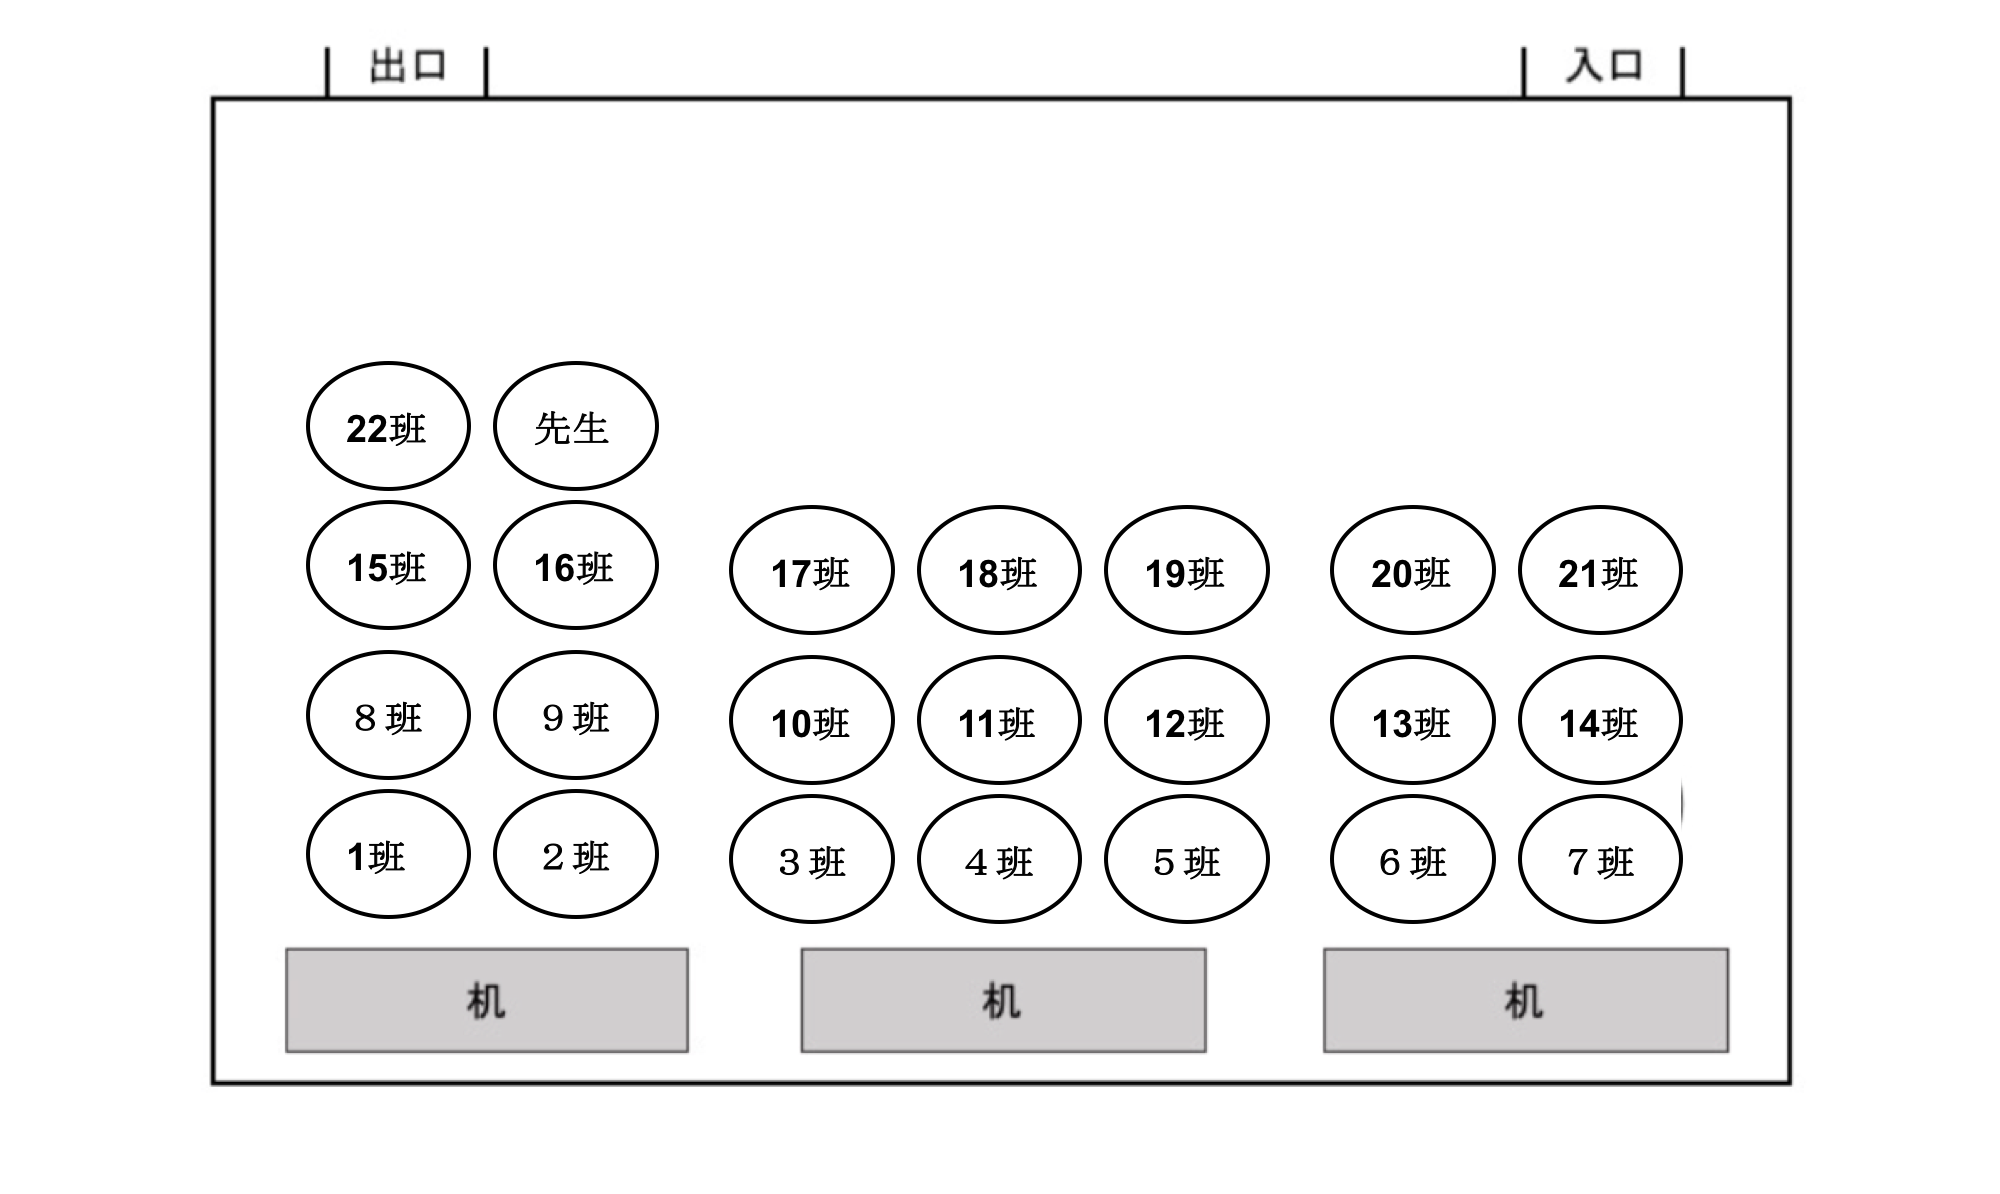
\includegraphics[width=100mm]{./03/nimotu.eps}
\end{center}
 \caption{第一集会室での荷物を置く配置}
 \label{fig:nimotsuhaichi}
\end{figure}

\newpage

\subsubsection{シーツ置き場}
\begin{figure}[htbp]
 \begin{center}
  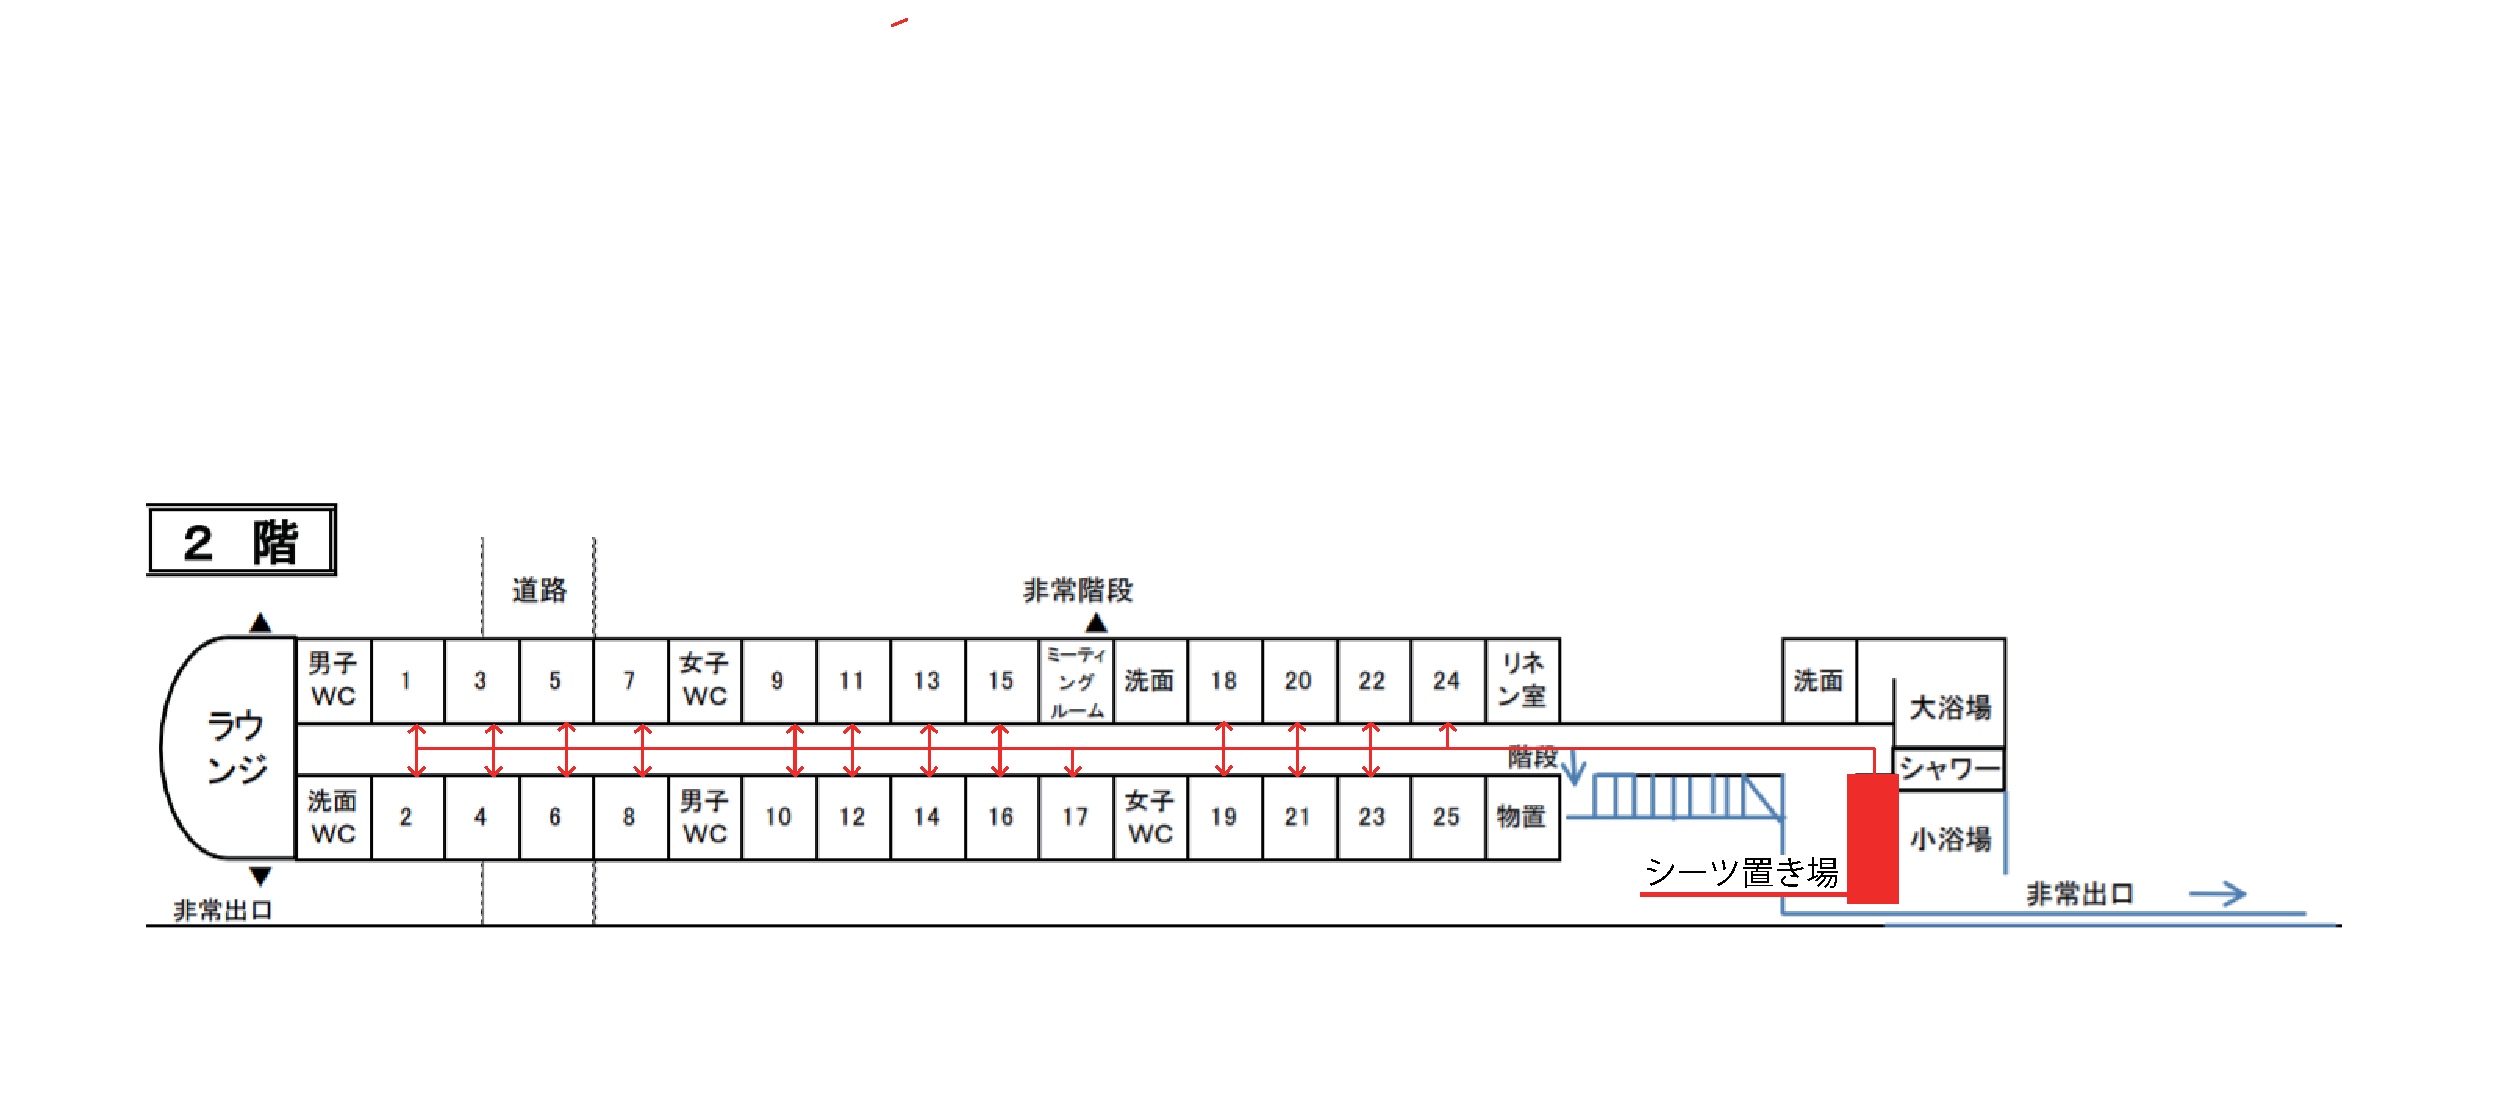
\includegraphics[width=90mm]{./03/situ.eps}
\end{center}
 \caption{シーツを置く位置}
 \label{fig:seatshaichi}
\end{figure}

\subsubsection{なかよし広間の配置}
\begin{figure}[htbp]
 \begin{center}
  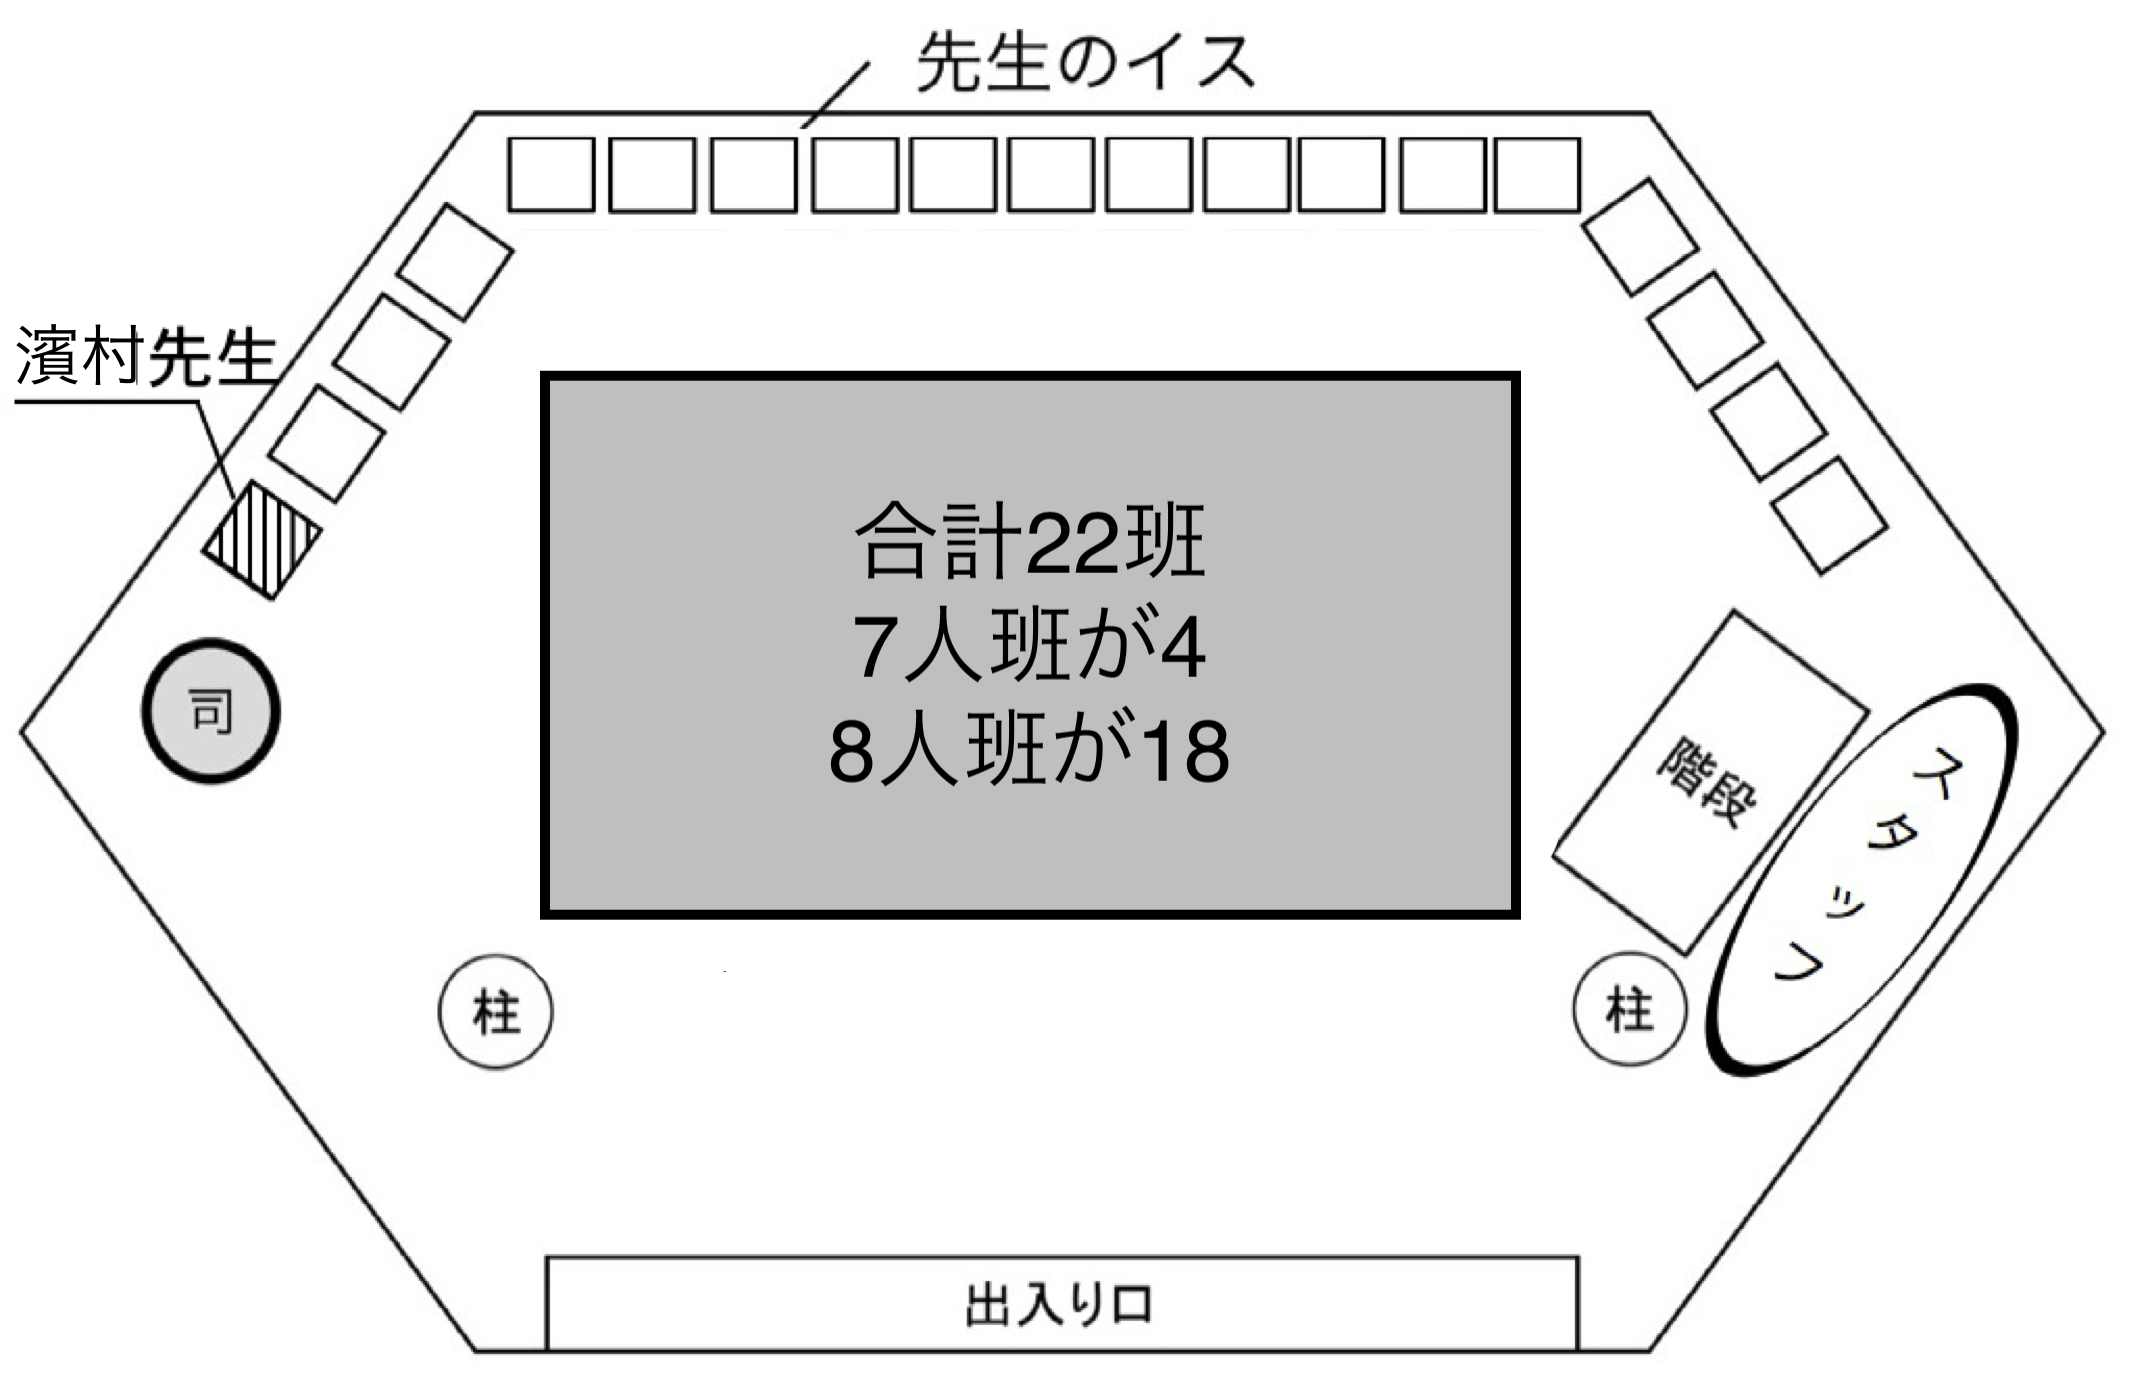
\includegraphics[width=100mm]{./03/nyushosiki.eps}
  \end{center}
 \caption{なかよし広間の配置}
 \label{fig:nakayoshihaichi}
\end{figure}

\newpage
\newpage
\subsubsection{なかよし広間誘導時の配置}
\begin{figure}[htbp]
  \begin{center}
   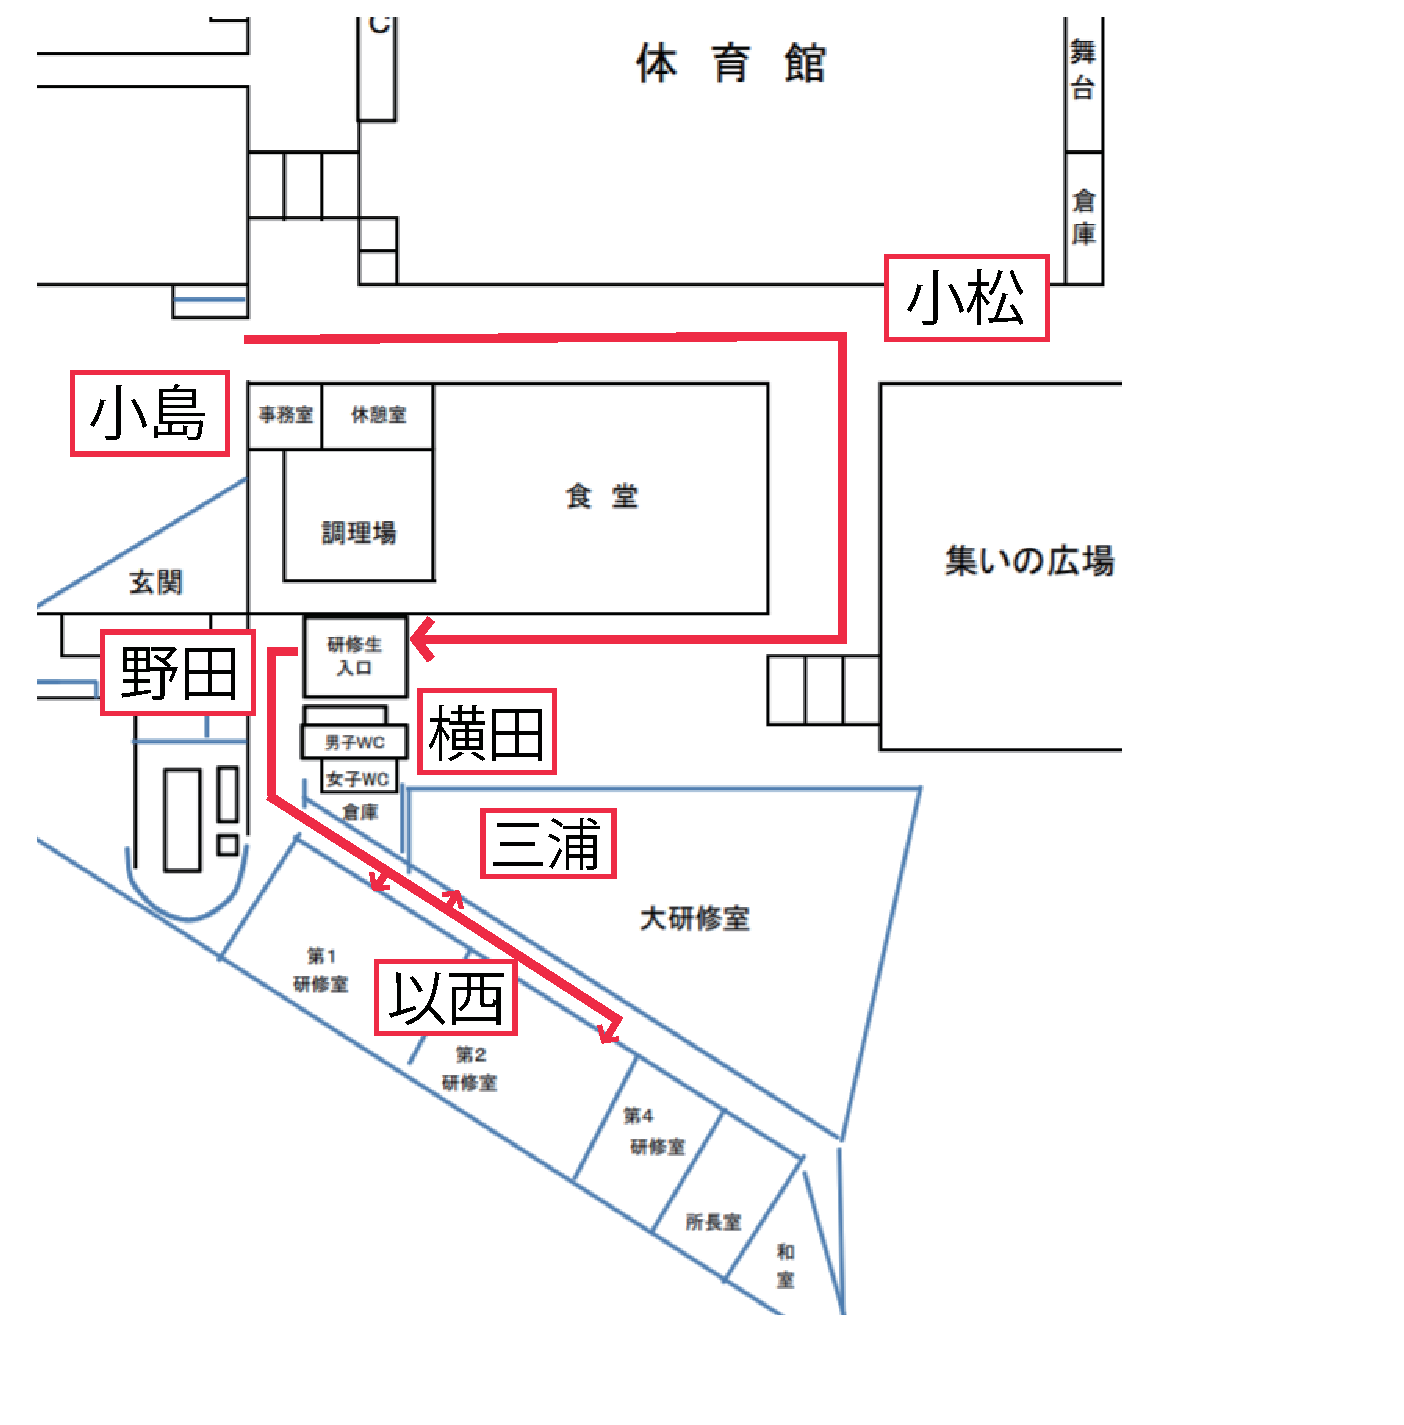
\includegraphics[width=140mm]{./03/yuudou.eps}
  \end{center}
  \caption{なかよし広間までの誘導 (晴天時)}
  \label{fig:hare}
\end{figure}

\begin{figure}[htbp]
  \begin{center}
   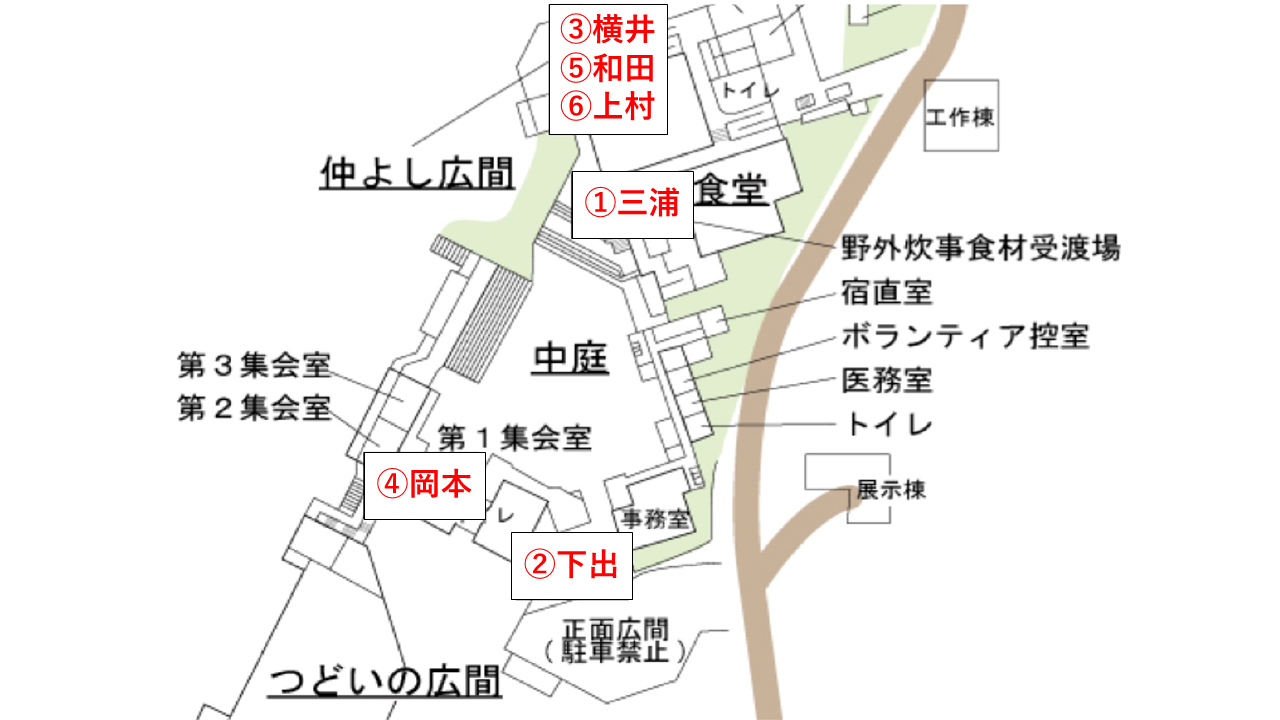
\includegraphics[width=120mm]{./03/yuudou2.eps}
  \end{center}
  \caption{なかよし広間までの誘導 (雨天時)}
  \label{fig:ame}
\end{figure}


\subsection{必要物品}
\begin{itemize}
\item 大研修室用の野外炊事班を示したプラカード:??枚
\item 第一・二研修室用の野外炊事班を示したプラカード:??枚
\item 野外炊事場用の野外炊事班を示したプラカード:??枚
\item 教員名を印刷した紙:??枚
\item マスキングテープ(イスに教職員名を貼り付ける用)
\item 野外炊事物品:予備(ピーラー,ふきん,着火剤,軍手,新聞紙,うちわ,チャッカマン),救急箱
%\item 靴入れビニール袋:200枚
%\item 傘袋:200枚
\item ブルーシート:1枚
\item マイク:2本
\item スピーカー:1台
\item 延長ケーブル
\item 救急箱 (大学の保健室から借りて持参)
\end{itemize}



\subsection{備考}
\begin{itemize}
\item バスの所在を随時連絡してもらうので時間を考えて行動する
\item 先遣隊で連絡を取り合い,終わっていないところの救援を行う
%\item 鍵の又貸しはせず,全ての場合に置いて鍵担当の岡本が鍵管理を行う
\item マイクの電池を確認しておく
\item 入所式に班名が書かれたプラカードを設置する
\end{itemize}


\subsection{連絡事項}
\begin{table}[h]
\begin{tabular}{|c|c|c|c|}
\hline
報告者 & 内容 & タイミング \\ \hline \hline
上村 & 先遣隊 (車2台) 到着 & 到着時\\ \hline
上村 & 準備完了 & 準備完了時 \\ \hline
\end{tabular}
\end{table}

%\include{end}
%%%%%%%%%%%%%%%%%%%%%%%%%%%%%%%%%%%%%%%%%%%%%%%%%%%%%%%%%%%%%%%%%%%%%%%%%%%%%%%
